%\makeatletter
%\global\let\tikz@ensure@dollar@catcode=\relax
%\makeatother
%
%\maketitle{}

\section{Cadre général.}

Soit avec $I$ un intervalle de $\R$ et $f: I\to\R$ une fonction.

On cherche à déterminer une approximation d'un $x\in I$ tel que $f(x)=0$, \emph{i.e.} d'une solution de l'équation $f(x) = 0$ (on parle aussi de \emph{zéro} de la fonction $f$).

%\clearslide{}
\section{Méthode dichotomique.}

C'est une méthode déjà vue en mathématiques. 
C'est par exemple une des méthodes permettant de démontrer le théorème des valeurs intermédiaires.

\subsection{Principe}

On suppose que $f$ est continue.

\begin{itemize}
\item On part de $a$ et $b$ ($a<b$) tels que $f(a)$ et $f(b)$ soient de signes
  contraires. Le TVI assure alors qu'il y a un point d'annulation de $f$ entre $a$ et $b$.
\item On calcule $m=\frac{1}{2}(a+b)$.
\item On itère en repartant de $a$ et $m$ ou de $m$ et $b$ en fonction
  du signe de $f(m)$.
\end{itemize}

%\clearslide{}
Pour savoir si on repart de $a$ et $m$ ou de $m$ et $b$:
\begin{itemize}
\item On considère le signe de $f(a)f(m)$.
\item Si $f(a)f(m) \leq 0$ : $f(a)$ et $f(m)$ sont de signes opposés, $f$ s'annule donc sur le segment $[a,m]$. On itère donc sur $[a,m]$.
\item Sinon, $f(a)f(m)>0$ : $f(a)$ et $f(m)$ sont de même signe, donc $f(m)$ et $f(b)$ sont
  de signes opposés, $f$ s'annule donc sur le segment $[m,b]$. On itère donc sur $[m,b]$.
\end{itemize}

\begin{rem}
  Si $f(a)f(m)=0$, $f(a)$ ou $f(m)$ est nul, on repart de $a$ et $m$ (on pourrait renvoyer directement $a$ ou $m$, 
mais, d'une part, dans la pratique, on ne tombe jamais exactement sur un point d'annulation et, d'autre 
part, à cause des erreurs de manipulations des flottants, un flottant n'est jamais vraiment égal à 0).
\end{rem}


%\clearslide{}

\subsubsection*{Invariant de l'algorithme}

Invariant de l'algorithme : à chaque itération,  $f(a)$ et $f(b)$ sont de signes opposés (donc
d'après le TVI il y a un point d'annulation de $f$ entre $a$ et $b$). C'est équivalent à : $f(a)f(b)\leq 0$.


%\clearslide{}

\subsubsection*{Terminaison}

On se donne un critère d'arrêt de boucle : on va demander à obtenir une valeur approchée du résultat à une précision $\varepsilon>0$ près. 

Pour un tel résultat à une précision $\varepsilon>0$, on
s'arrête quand $b - a \leq 2\varepsilon$ et on renvoie $\frac{a+b}{2}$.
On obtient bien une valeur approchée à $\varepsilon>0$ près. 

Comme l'écart $b-a$ suit une progression géométrique de raison
  $\frac{1}{2}$, donc tend vers $0$, l'algorithme s'arrête (après un nombre fini d'itérations).

%\clearslide{}
\subsection{Implantation}
% \small{}
\begin{lstlisting}
def dichotomie(f, a, b, epsilon):
    """Zéro de f sur [a,b] à epsilon près, par dichotomie
       Préconditions : f(a) * f(b) <= 0
                       f continue sur [a,b]
                       epsilon > 0"""
    c, d = a, b
    fc, fd = f(c), f(d)
    while d - c > 2 * epsilon:
        m = (c + d) / 2.
        fm = f(m)
        if fc * fm <= 0:
            d, fd = m, fm
        else:
            c, fc = m, fm
    return (c + d) / 2.
\end{lstlisting}
% \normalsize{}
%\clearslide{}
\begin{rem}
  On a pris soin ici de réaliser le moins possible d'appels à la fonction $f$.
\end{rem}

\begin{rem}
  Comme on connait le nombre exact d'itérations, on aurait aussi pu écrire une boucle \texttt{for}. La fonction en perdrait alors en lisibilité. 
\end{rem}
%\clearslide{}

\subsection{Démonstration}

\begin{description}
\item[Terminaison~:] le variant est $\ceil{\log_{2}\p{\frac{d-c}{\varepsilon}}} - 1$, qui diminue de un à chaque tour de 
boucle. Comme c'est un entier, il devient nul ou négatif en un nombre fini de tours de boucle. Or il est négatif ou nul 
si et seulement si $\log_{2}\p{\frac{d-c}{\varepsilon}}\leq 2$, si et seulement si $d-c \leq 2\varepsilon$, ce qui est 
la condition d'arrêt de la boucle \pyv{while}.
\item[Correction~:] l'invariant est~: \og $f(c).f(d)\leq 0$, donc $f$ possède un point d'annulation entre $c$ et $d$\fg. Il 
se démontre aisément par récurrence. Ainsi, après la boucle \pyv{while}, $f$ possède un point d'annulation entre $c$ 
et $d$, et la distance entre $c$ et $d$ est inférieure à $2\varepsilon$. L'algorithme renvoie $(c+d)/2$, qui est 
nécessairement à une distance d'un point d'annulation inférieure à $\varepsilon$.
\end{description}



%\clearslide{}
\subsection{Complexité}

Le nombre de tours de boucle est
\begin{equation*}
  \ceil{\log_{2}\p{\frac{b-a}{\varepsilon}}} - 1.
\end{equation*}

Ainsi, pour avoir $p$ bits significatifs, $\Theta(p)$ tours de
boucle sont effectués.

\emph{NB} : en écrivant cet algorithme, une attention a été portée aux calculs des valeurs de $f$~: on a évité de calculer 
plusieurs fois la même valeur. Cela ne change rien à la complexité asymptotique, mais peut avoir une importance en 
pratique.

%\clearslide{}

\subsection{Avantages et inconvénients}

\textbf{Avantages~:} la convergence théorique est assurée et nous avons une bonne idée de l'erreur (division 
par deux à chaque étape). De plus, les hypothèses sur $f$ sont faibles.\\

%\clearslide{}
\textbf{Inconvénients~:}
\begin{itemize}
\item la convergence n'est pas si rapide, comparée à d'autres méthodes (un bit significatif de 
plus à chaque étape).
\item si l'une des deux bornes de l'intervalle de départ est très proche d'un point d'annulation, 
la convergence ne sera pas plus rapide pour autant.
\item elle ne permet pas de trouver d'approximation pour un point d'annulation où le graphe de $f$ 
est tangente à l'axe des abscisses, car $f$ n'y change pas de signe.
\item Problèmes numériques~: si les valeurs manipulées sont trop petites, on peut avoir
$f(a)\times f(b)$ nul avec $f(a)\neq 0$ et $f(b)\neq 0$. Le logiciel peut aussi donner $f(b)<0$ 
alors qu'en réalité $f(b)>0$. Dans ce cas la mauvaise moitié est choisie et on peut aboutir à une 
approximation très éloignée de la réalité.
\end{itemize}

Cette méthode est intéressante pour avoir rapidement une première approximation, et se trouver en 
position d'utiliser ensuite une méthode plus performante.

%\clearslide{}
\section{Méthode de Newton (ou de Newton-Raphson)}

\subsection{Un exemple}
Voyons-en graphiquement  le principe sur l'exemple de $f:x\mapsto x^{2} -2$.

\begin{center}
 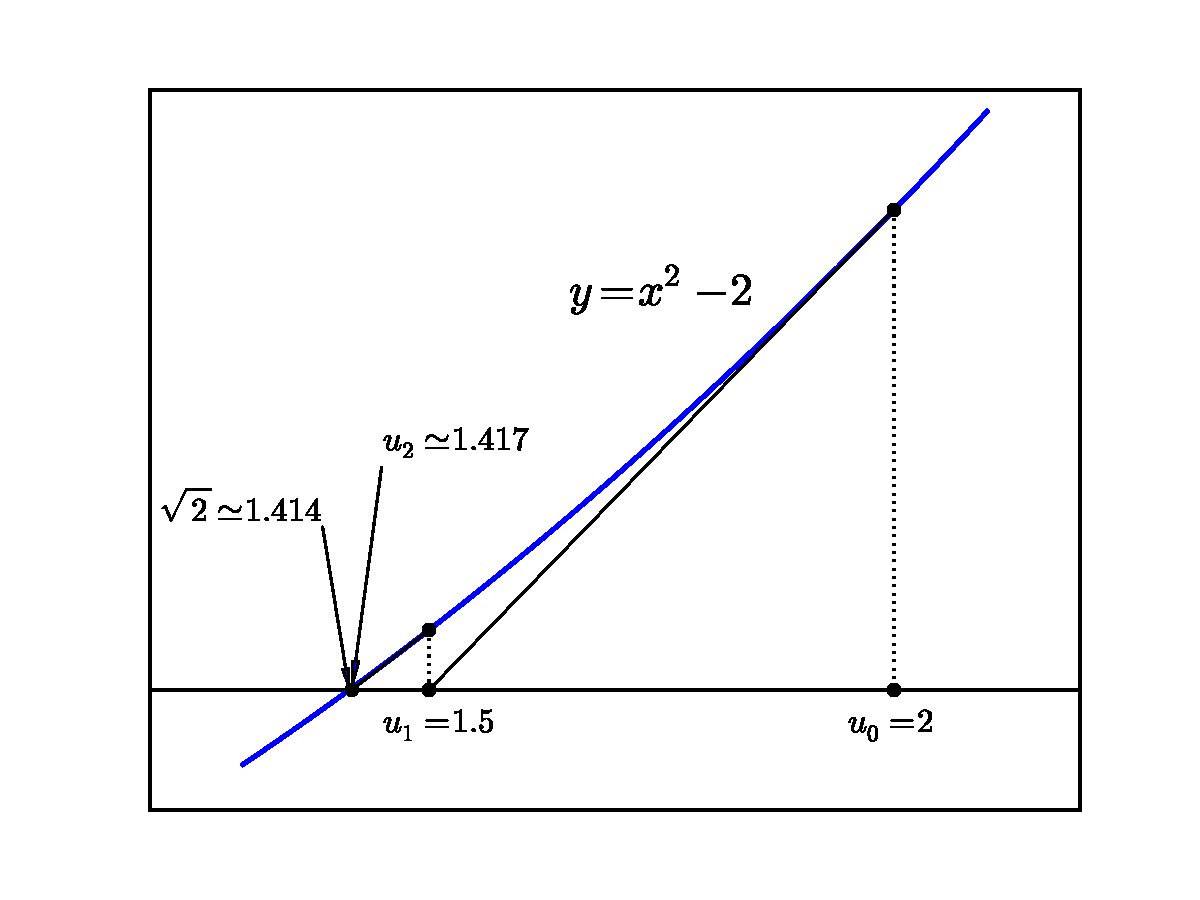
\includegraphics[width=0.8\textwidth]{newton.pdf}
\end{center}

%\clearslide{}
\subsection{Définition}

Cette méthode est \emph{itérative}~: on construit une suite $\p{u_{n}}_{n\in\N}$ telle que~:
\begin{itemize}
\item $u_{0}$ est une approximation d'un zéro de $f$, souvent grossière.
\item On pose, pour $n\in\N$, $u_{n+1}=F(u_{n})$, où 
  $F : x\mapsto x - \dfrac{f(x)}{f'(x)}$.
  
Ainsi, le point $(u_{n+1},0)$ est le point d'intersection de l'axe des abscisses et de la 
tangente à la courbe de $f$ en $u_n$.
\end{itemize}
\begin{center}
 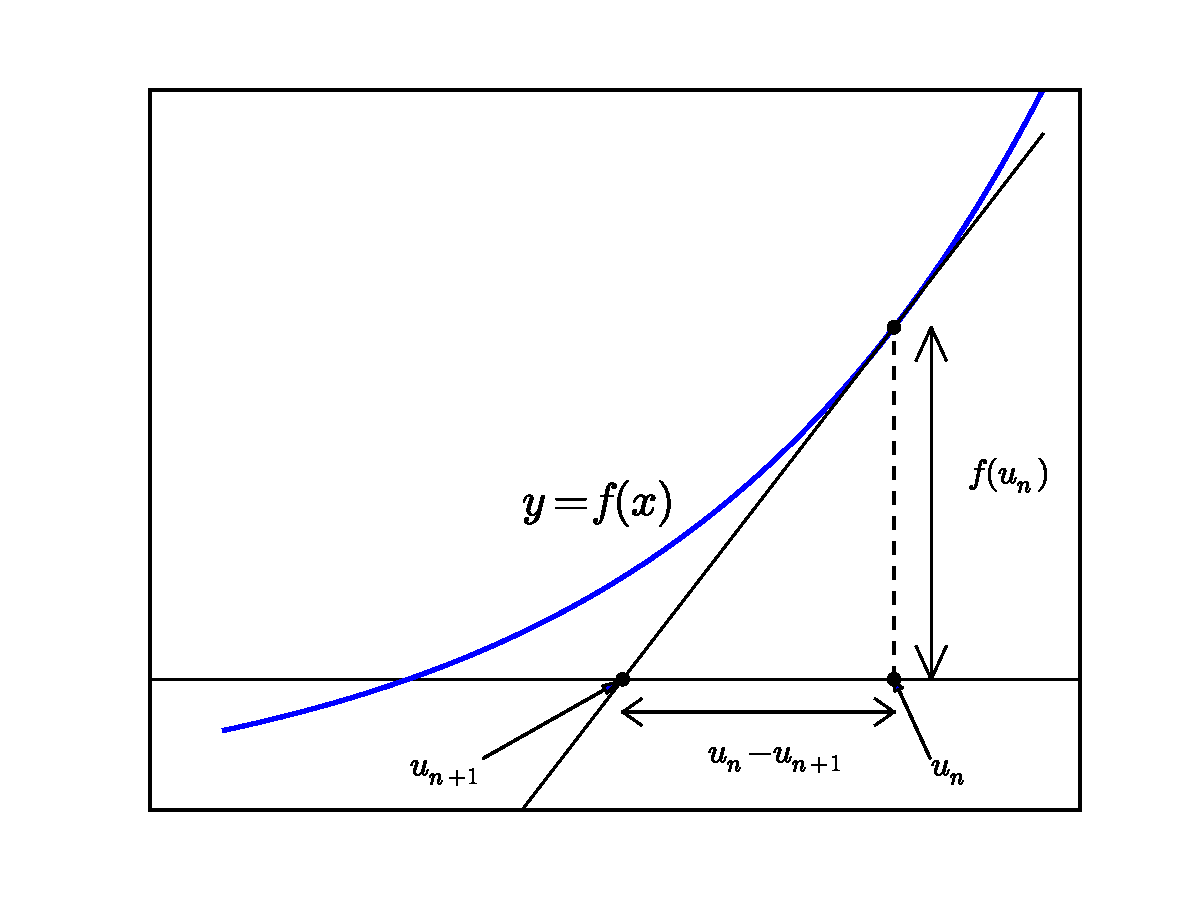
\includegraphics[width=0.7\textwidth]{newton-generique.pdf}
\end{center}
%\clearslide{}
\subsection{Implantation}
\begin{lstlisting}
def newton(f, fp, x0, epsilon):
    """Zéro de f par la méthode de Newton
       départ : x0, f' = fp, critère d'arrêt epsilon"""
    u = x0
    v = u - f(u)/fp(u)
    while abs(v-u) > epsilon:
        u, v = v, v - f(v)/fp(v)
    return u
\end{lstlisting}
%\clearslide{}
\subsection{Correction, terminaison, complexité.}

Se posent notamment les problèmes suivants.
\begin{enumerate}
\item La suite est-elle bien définie ? Plus précisément, évite-t-on les divisions par zéro ? La dérivée $f'$ 
s'annule-t-elle ?
\item L'algorithme se termine-t-il ? La suite converge-t-elle ? 
\item Le résultat est-il proche d'un zéro de $f$ ?
\end{enumerate}

\begin{rem}
  Le deuxième point n'est pas assuré. Plusieurs problèmes peuvent se poser, notamment : 
  \begin{itemize}
    \item point singulier au point d'annulation (exemple : $x\mapsto\sqrt{|x|}$, réalisez le calcul à la main) ;
    \item point initial éloigné du zéro.
  \end{itemize}
\end{rem}


%\clearslide{}
\subsubsection{Mathématiquement.}

Soit $x_{0}\in I$ tel que $f(x_{0}) = 0$.

Supposons que 
\begin{itemize}
\item $f$ est de classe $\mathcal{C}^{2}$ ;
\item $f'(x_{0})\neq 0$.
\end{itemize}

Alors, pour $u_{0}$ suffisamment proche
de $x_{0}$, il existe $C>0$ tel que
\begin{equation*}
  \forall n\in\N\quad \abs{u_{n} - x_{0}} \leq C 2^{-2^{n}}.
\end{equation*}

Le nombre de chiffres corrects \emph{double} à chaque itération !

De plus, l'impact des erreurs de calcul est généralement faible (c'est souvent l'intérêt d'une
méthode itérative).
%\clearslide{}
\subsubsection{Démonstration}

Pour $h$ au voisinage de $0$:
\begin{align*}
 f(x_{0}+h) &= f(x_{0}) + hf'(x_{0}) + f''(x_{0})h^{2} + o(h^{2})\\
 &= hf'(x_{0}) + O(h^{2})
\end{align*}
et 
\begin{align*}
 f'(x_{0}+h)&= f'(x_{0}) + hf''(x_{0}) + o(h)\\
 &= f'(x_{0}) + O(h).
\end{align*}
Ainsi,
\begin{align*}
F(x_{0}+h) &= x_{0} + h - \frac{hf'(x_{0})+O(h^{2})}{f'(x_{0})+O(h)}\\
&= x_{0} + h - \frac{hf'(x_{0})}{f'(x_{0})}\times\frac{1+O(h)}{1+O(h)}\\
&= x_{0} + h - h\times(1+O(h))\\
&= x_{0} + O(h^{2}).
\end{align*}
%\clearslide{}
Autrement dit, au voisinage de $x_0$,
\begin{equation*}
  F(x) = x_{0} + O\p{\p{x-x_{0}}^{2}}.
\end{equation*}
Il existe donc des constantes $\alpha>0$ et $K>0$ vérifiant
\begin{equation*}
  \forall x\in [x_{0}-\alpha, x_{0}+\alpha],
  \quad \abs{F(x) - x_{0}}\leq K\abs{x-x_{0}}^{2}.
\end{equation*}
%\clearslide{}
On peut supposer $K\alpha<\frac{1}{2}$ (quitte à diminuer $\alpha$).

Alors :
\begin{itemize}
\item $[x_{0}-\alpha, x_{0}+\alpha]$ est stable par $F$ ;
\item $\forall n\in\N,\quad K\abs{u_{n+1}-x_{0}}\leq \p{K\abs{u_{n}-x_{0}}}^{2}$.
\end{itemize}
Par une récurrence simple, on obtient directement que, pour tout $n\in \N$,
\begin{align*}
  K\abs{u_{n}-x_{0}}&\leq  (K\abs{u_{0}-x_{0}})^{2^{n}}\\
                    &\leq (K\alpha)^{2^n}\\
                    &\leq 2^{-2^{n}}.
\end{align*}

%\clearslide{}
\subsubsection{En pratique}
% \begin{center}
%   \includegraphics[width=0.7\textwidth]{precision-newton.pdf}
% \end{center}

On donne sur la figure \ref{precision} les erreurs d'approximation selon la méthode utilisée.

\begin{figure}[!h]
\begin{center}
  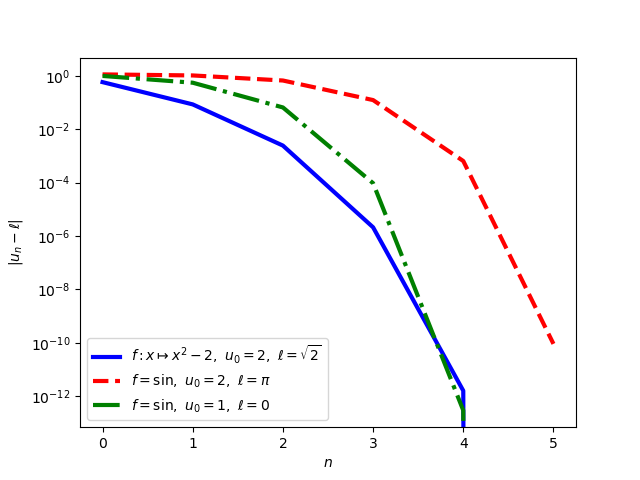
\includegraphics[width=\textwidth]{precision_newton.png}
  \caption{Erreurs d'approximation de zéros de trois fonctions ($f$), par la méthode de Newton (point initial : $u_0$). Échelle semi-logarithmique. \label{precision}}
\end{center}
\end{figure}
\subsection{Applications}
\subsubsection{Au calcul de $1/a$ ($a>0$)}

Les calculs du rapport de deux flottants ou de l'inverse d'un flottant sont parmi les opérations les plus 
difficiles à calculer sur un processeur. Une méthode fréquente consiste à implanter un micro-logiciel de calcul dans le 
processeur.\\

%\clearslide{}
On calcule une première approximation $u_{0}$ de l'inverse de $a$, puis on applique la méthode de Newton à la fonction
$f: x\mapsto \frac{1}{x} - a$. On pose donc~:

\begin{equation*}
  u_{n+1} = u_{n} - \frac{f(u_{n})}{f'(u_{n})}
  = u_{n} + u_{n} - a  u_{n}^{2} = u_{n}(2 - au_{n}).
\end{equation*}

%\clearslide{}
\subsubsection{Au calcul de la racine carrée (version matheuse)}

On applique la méthode de Newton à la fonction
$f:x\mapsto x^{2} -a$, où $a>0$ est le nombre dont on veut la racine
carrée~:
\begin{equation*}
  u_{n+1} = u_{n} - \frac{u_{n}^{2}-a}{2u_{n}}
  = \frac{1}{2}\p{u_{n}+\frac{a}{u_{n}}}
\end{equation*}

Cette méthode fonctionne correctement sur le papier mais nécessite un calcul d'inverse à chaque étape
(plus deux multiplications, une addition et une division par deux).
%\clearslide{}
\subsubsection{Au calcul de la racine carrée (version
  informaticienne)}
On applique la méthode de Newton à la fonction
$f:x\mapsto \frac{1}{x^{2}} -a$, où $a>0$ est le nombre dont on veut
la racine carrée~:
\begin{equation*}
  u_{n+1} = u_{n} - \frac{\frac{1}{u_{n}^{2}}-a}{-\frac{2}{u_{n}^{3}}}
  = \frac{1}{2}u_{n}\p{3 - au_{n}^{2}}.
\end{equation*}

On multiplie l'approximation de $\frac{1}{\sqrt{a}}$ obtenue par $a$
pour obtenir une approximation de $\sqrt{a}$.

%\clearslide{}
Dans les jeux vidéos les calculs d'inverses et de racines carrées sont très utilisés, en particulier pour les calculs 
d'angles d'incidence et de réflexion (calcul des
  lumières et des ombres en imagerie numérique). Pour cela on a besoin de normaliser des vecteurs ( \emph{i.e.} 
calculer $\vec{u}/{\Vert\vec{u}}\Vert$), on a donc besoin de calculer l'inverse d'une racine carrée. Cela a ammené la création de la
méthode \emph{Fast inverse square root}~: développée vers 1990 chez Silicon Graphics (probablement), elle a par exemple 
été utilisée dans Quake III Arena (1999), et elle utilise la méthode de Newton.

%\clearslide{}
\subsection{Calcul approché de la dérivée}

Pour effectuer la méthode de Newton, on a besoin de connaître $f'$.

Un moyen de la calculer numériquement est d'utiliser l'approximation suivante~:
\begin{equation*}
  \frac{f(x_{0}+h)-f(x_{0})}{h}\approx f'(x_{0}) \quad\text{(pour $h$ petit)}.
\end{equation*}

L'erreur commise est $\frac{h}{2}f''(x_{0}) + o(h)$ (si $f$ est de classe
$\mathcal{C}^{2}$).\\


%\clearslide{}
En voici une approximation plus précise (et pas plus dure à calculer)~:
\begin{equation*}
    \frac{f(x_{0}+h)-f(x_{0}-h)}{2h} = f'(x_{0}) +
    \frac{h^{2}}{6}f^{(3)}(x_0)+o(h^{2})
    \quad\text{(si $f$ est de classe $\mathcal{C}^{3}$)}.
\end{equation*}\\


%\clearslide{}

\subsection{Méthode de la sécante}
Si l'on ne connaît pas la dérivée de $f$, et que l'on ne souhaite pas l'approcher (dans le cas d'une fonction peu régulière, par exemple), on peut remplacer la tangente à la courbe de $f$ par la corde à la courbe de $f$ entre deux points. 

On choisit deux approximations initiales $u_{0}$ et $u_{1}$ et on calcule l'intersection de la corde à la courbe de $f$ entre les points d'abscisses $u_0$ et $u_1$ avec l'axe des abscisses. 
On note $u_2$ l'abscisse de ce point d'intersection, et on itère avec $u_1$ et $u_2$...
%\clearslide{}
\begin{rem}
  La corde à la courbe de $f$ entre les points d'abscisses $u_n$ et $u_{n-1}$ a pour pente $\dfrac{f(u_{n})-f(u_{n-1})}{u_{n}-u_{n-1}}$ et a donc pour équation : 
  \begin{align*}
    y &= f(u_n) + (x-u_n)\dfrac{f(u_{n})-f(u_{n-1})}{u_{n}-u_{n-1}} \\
      &= f(u_{n-1}) + (x-u_{n-1})\dfrac{f(u_{n})-f(u_{n-1})}{u_{n}-u_{n-1}}.
  \end{align*}
\end{rem}
On considère donc la suite définie par récurrence par : 
\begin{equation*}
  \forall n\in\N^{*} \quad u_{n+1} = u_{n} -
  f(u_{n})\frac{u_{n}-u_{n-1}}{f(u_{n})-f(u_{n-1})}.
\end{equation*}

%\clearslide{}
\begin{center}
\resizebox{0.6\textwidth}{!}{\input{images/secante.pdf_t}}
\end{center}

%\clearslide{}
En Python, cela donne une fonction très proche de celle écrite pour la méthode de Newton. 
\begin{lstlisting}
def secante(f,u0,u1,eps):
    """Zéro de f par la méthode de la sécante
    u0,u1 : deux premiers points
    eps : critère d'arrêt"""
    u,v = u0,u1
    while abs(u-v) > eps : 
        p = (f(u)-f(v)) / (u-v)
        u,v = v,u - f(u)/p
    return u
\end{lstlisting}

%\clearslide{}

On peut montrer que si $u_{0}$ et $u_{1}$ sont suffisamment proches du
zéro cherché et si $f$ est de classe $\mathcal{C}^{2}$, il existe $C>0$ tel que
\begin{equation*}
  \forall n\in\N\quad \abs{u_{n} - x_{0}} \leq C 2^{-(\frac{1+\sqrt5}2)^{n}}.
\end{equation*}
Voir la figure~\ref{12resolution-eq:fig:comp_sec_newton} pour une illustration.



%\clearslide{}

\begin{figure}[!h]
\begin{center}
  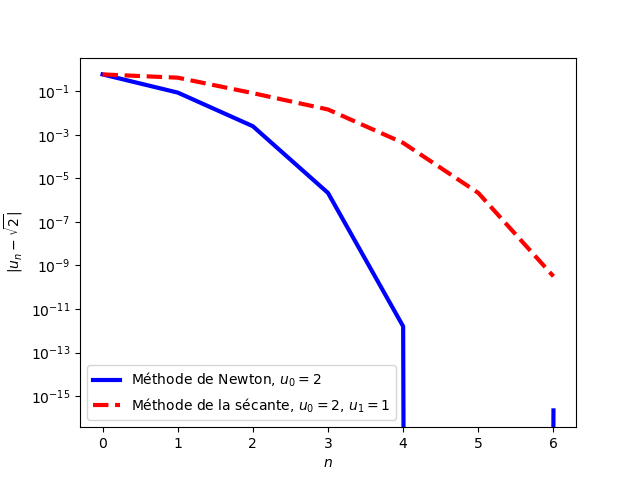
\includegraphics[width=\textwidth]{comparaison_newton_secante.png}
  \caption{Erreurs d'approximation du zéro de $x\mapsto x^2-2$ par la méthode de Newton et la méthode de la sécante. Échelle semi-logarithmique.}
  \label{12resolution-eq:fig:comp_sec_newton}
\end{center}
\end{figure}

%\clearslide{}
\section{Méthodes proposées par numpy et scipy}
Intérêt de l'utilisation de numpy et scipy~: ne pas réinventer l'eau
chaude.
\subsection{Racines d'un polynôme}
Pour calculer les racines de
\begin{equation*}
 P = \sum_{k=0}^{n}a_{k}X^{k}
\end{equation*}
on utilise
\begin{lstlisting}
numpy.roots([a0, a1, ..., an])
\end{lstlisting}
Exemple:
\begin{pyconsole}
import numpy
numpy.roots([2, 0, 1])
\end{pyconsole}

Quelle est la méthode employée?
%\clearslide{}

La plupart des utilisateurs utilisent \pyv{numpy.roots} sans se
poser de questions.

Mais il y a des cas où nous avons besoin d'avoir une idée de l'erreur:
\begin{enumerate}
\item On peut essayer de tester expérimentalement (mais comment être
  exhaustif?);
\item On peut enquêter pour trouver la réponse.
\end{enumerate}

Enquêtons\ldots{}
%\clearslide{}

La documentation (\pyv{help(numpy.roots)}) nous dit notamment:
\begin{quote}
the algorithm relies on computing the eigenvalues of the
companion matrix [1].

[1] r. a. horn \& c. r. johnson, \emph{matrix analysis}.  cambridge, uk:
    cambridge university press, 1999, pp. 146-7.
\end{quote}
Pour continuer : consulter la bibliothèque universitaire la plus proche.
\medskip
%\clearslide{}

Mais par quelle méthode calcule t-on ces valeurs propres ?
Le code nous renseigne :
\begin{lstlisting}
a = diag(nx.ones((n-2,), p.dtype), -1)
a[0, :] = -p[1:] / p[0]
roots = eigvals(a)
\end{lstlisting}
On construit une matrice $a$ nulle à l'exception de la sous-diagonale
(où on met des $1$), puis on remplace la première ligne par les
coefficients $-\frac{a_{1}}{a_{0}}, \ldots, -\frac{a_{n}}{a_{0}}$ et
on calcule les valeurs propres (\textit{eigenvalues}) de la matrice
obtenue.

Vous en comprendrez la raison après avoir étudié un peu plus d'algèbre linéaire (voir les \emph{matrices compagnon}).

\medskip

%\clearslide{}
Allons donc voir \pyv{help(numpy.linalg.eigvals)} :
\begin{quote}
This is a simple interface to the LAPACK routines dgeev and zgeev
that sets those routines' flags to return only the eigenvalues of
general real and complex arrays, respectively.
\end{quote}

Qu'est-ce que LAPACK ? D'après Wikipédia, c'est l'acronyme de \emph{Linear Algebra Package} : 
\begin{quote}
LAPACK (pour Linear Algebra PACKage) est une bibliothèque logicielle
écrite en Fortran, dédiée comme son nom l'indique à l'algèbre linéaire
numérique.
\end{quote}
Mais quelle est la \emph{méthode} employée?

En utilisant  un moteur  de recherche («LAPACK  dgeev»), on  trouve un
fichier  \texttt{dgeev.f} (fichier  FORTRAN)  dont la  doc évoque  une
décomposition  QR... sans  vraiment  faire référence  à un  algorithme
précis.
\bigskip

%\clearslide{}
Conclusion: il s'agit plus d'une quête que d'une enquête.
\begin{itemize}
\item Les algorithmes utilisés sont souvent subtils et font appels à
  des mathématiques relativement évoluées.
\item Il est difficile de  savoir exactement ce qu'il se  passe sous le
capot.
\item On peut quand même aller lire le code de \texttt{dgeev}.
\item Heureusement, il est public\ldots{} 
\item Wikipédia est  en général un bon point  d'entrée pour débuter la
  quête (ici \emph{QR algorithm} sur \texttt{http://en.wikipedia.org}).
\end{itemize}

%\clearslide{}
\subsection{Méthode de Newton/de la sécante}
Recherche d'un zéro d'une fonction:

\pyv{scipy.optimize.newton(func, x0, fprime)}

La documentation est claire:
\begin{quote}
  Find a zero using the Newton-Raphson or secant method.

  Find a zero of the function `func` given a nearby starting point `x0`.
  The Newton-Raphson method is used if the derivative `fprime` of `func`
  is provided, otherwise the secant method is used.
\end{quote}

%\clearslide{}
\subsection{Méthode de Brent}

\pyv{scipy.optimize.brentq(f, a, b)}.

La qualité de la documentation est remarquable.

Ça commence par dire \emph{ce que} ça fait:

\begin{quote}
Find a root of a function in given interval.

Return float, a zero of `f` between `a` and `b`.  `f` must be a continuous
function, and [a,b] must be a sign changing interval.
\end{quote}

%\clearslide{}
Puis ça continue par \emph{comment} ça le fait:
\begin{quote}
Description:
Uses the classic Brent (1973) method to find a zero of the function `f` on
the sign changing interval [a , b].  Generally considered the best of the
rootfinding routines here.  It is a safe version of the secant method that
uses inverse quadratic extrapolation.  Brent's method combines root
bracketing, interval bisection, and inverse quadratic interpolation.  It is
sometimes known as the van Wijngaarden-Deker-Brent method.  Brent (1973)
claims convergence is guaranteed for functions computable within
[a,b].
\end{quote}

%\clearslide{}
Puis \emph{comment trouver plus d'information} (la référence
historique et des références plus faciles d'accès):
\begin{quote}
[Brent1973] provides the classic description of the algorithm.  Another
description can be found in a recent edition of Numerical Recipes, including
[PressEtal1992].  

Another description is at
http://mathworld.wolfram.com/BrentsMethod.html.  

It should be easy to
understand the algorithm just by reading our code.  Our code diverges a bit
from standard presentations: we choose a different formula for the
extrapolation step.

[Brent1973]
   Brent, R. P.,
   \emph{Algorithms for Minimization Without Derivatives}.
   Englewood Cliffs, NJ: Prentice-Hall, 1973. Ch. 3-4.

[PressEtal1992]
   Press, W. H.; Flannery, B. P.; Teukolsky, S. A.; and Vetterling, W. T.
   \emph{Numerical Recipes in FORTRAN: The Art of Scientific Computing}, 2nd ed.
   Cambridge, England: Cambridge University Press, pp. 352-355, 1992.
   Section 9.3:  "Van Wijngaarden-Dekker-Brent Method."
\end{quote}

%\clearslide{}
\section{Choisir une méthode}

Le choix de la méthode à utiliser dépend de différents facteurs. 
\begin{itemize}
\item Peut-on utiliser un programme existant ou doit-on programmer une
  méthode soi-même ?
\item La méthode doit-elle s'appliquer à une large classe de fonctions
  (par exemple pas nécessairement dérivables) ou à quelques fonctions
  régulières et bien identifiées ?
\item Dispose t-on d'une expression de la dérivée ?
\item Cherche t-on une solution dans un intervalle bien précis ou
  n'importe quelle solution ?
\item A t-on besoin d'une convergence rapide ?
\end{itemize}

Suivant les cas, on choisira la méthode :
\begin{itemize}
\item de dichotomie;
\item des sécantes;
\item de Brent;
\item ou de Newton.
\end{itemize}

Vous devez être capables de mettre en {\oe}uvre \emph{vous-même} la méthode de la dichotomie ainsi que celle de Newton. 
Commencez par vous exercer sur les exemples vus en cours ! 

%\section{Exercices}
%
%%\begin{exo}
%  On rappelle que $\cos\left(\frac{\pi}{10}\right)$ est une des solutions de l'équation $16x^4-20x^2+5 = 0$. En déterminer une valeur approchée à $10^{-10}$ près.
%%\end{exo}
%
%%\begin{exo}
%  Déterminer une valeur approchée du nombre d'or à $10^{-10}$ près.
%%\end{exo}
%
%%\begin{exo}
%  Écrire une fonction déterminant, pour tout $p \in \N^\ast$, une valeur approchée de l'équation $1 = x + x^2 + \dots + x^p$. 
%%\end{exo}



